\section{Exercise 2: Tracers of deep ocean circulation change}
\label{sec:E2}

\subsection{Question 1}
\label{sec:Q2.1}
See Figure \ref{fig:age_depth}

\begin{figure}[!htbp]
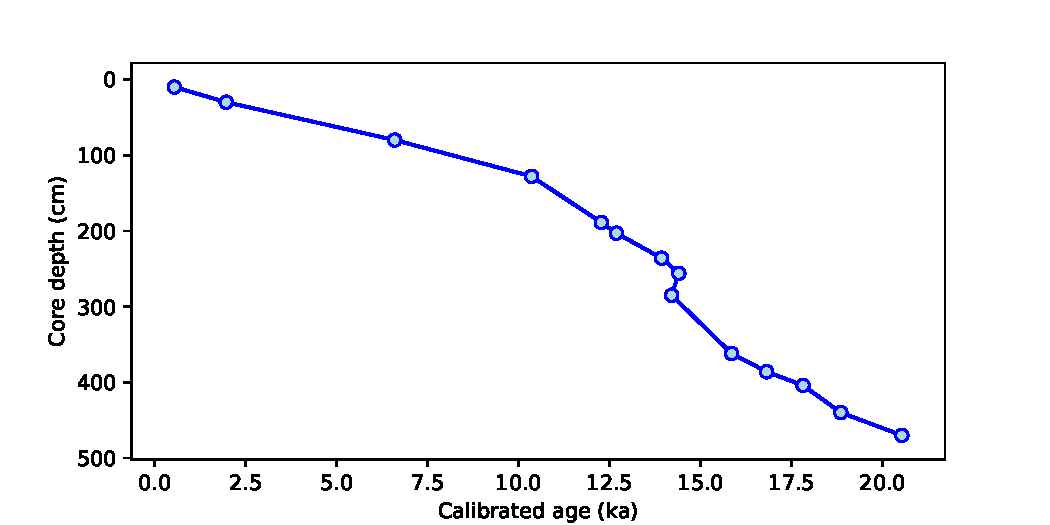
\includegraphics[width=\textwidth]{img/line_age_depth.pdf}
    \caption{Planktic foraminifera calibrated age against depth in sediment core OCE-326-GGC14, on the Laurentian fan.}
        \label{fig:age_depth}
\end{figure}

\subsection{Question 2}
\label{sec:Q2.2}

\begin{figure}[!htbp]
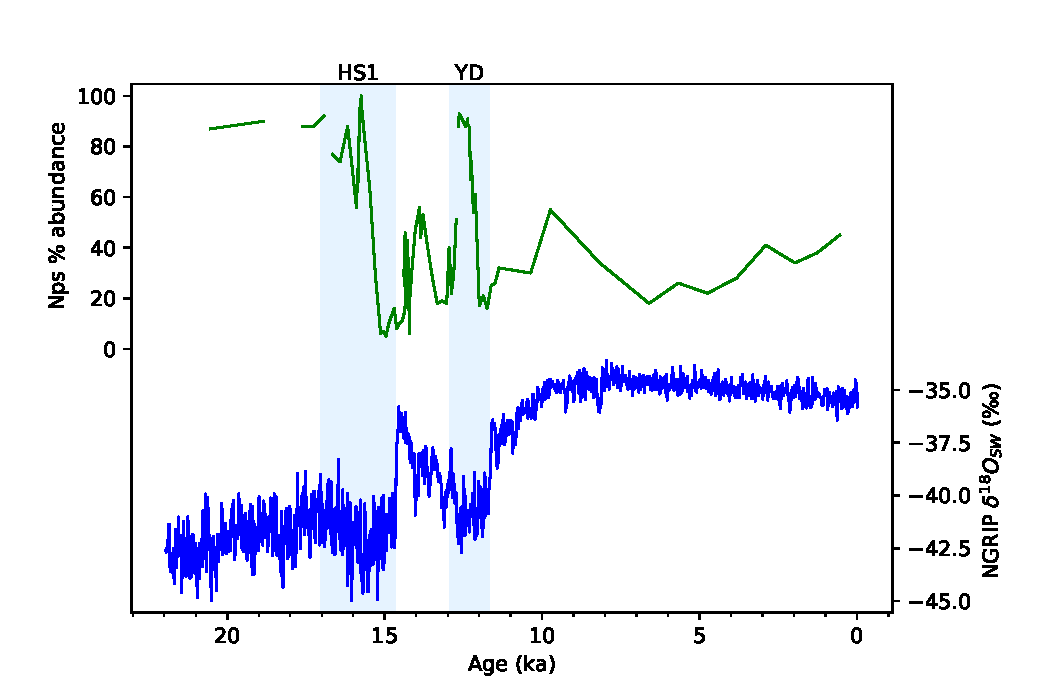
\includegraphics[width=\textwidth]{img/timeseries_nps_ngrip}
    \caption{Time series of abundance of planktic foraminifera \emph{N. pachyderma} sinistral (\emph{Nps}) in OCE-326-GGC14 (top) and oxygen isotope excursion in Greenland ice core NGRIP (bottom).}
        \label{fig:nps_ngrip}
\end{figure}

Figure \ref{fig:nps_ngrip} shows a strong antiphase relationship between \emph{Nps} abundance in the North Atlantic and \delO{} in Greenland, and both record abrupt climate cooling during the HS1 and YD stadials.
While changes in the latter appear to lag those in the former by approximately 0.5--1 ka, there is uncertainty in the calibration of foraminiferal \fC{} radiocarbon dates due to measurement error and, in particular, the assumption of a constant 400 year radiocarbon reservoir age --- a value that was likely higher during stadial events due to decreased ocean ventilation \parencite{bard1994north, hughen2004marine04}.

            
\subsection{Question 3}
\label{sec:Q2.3}
\begin{figure}[p]
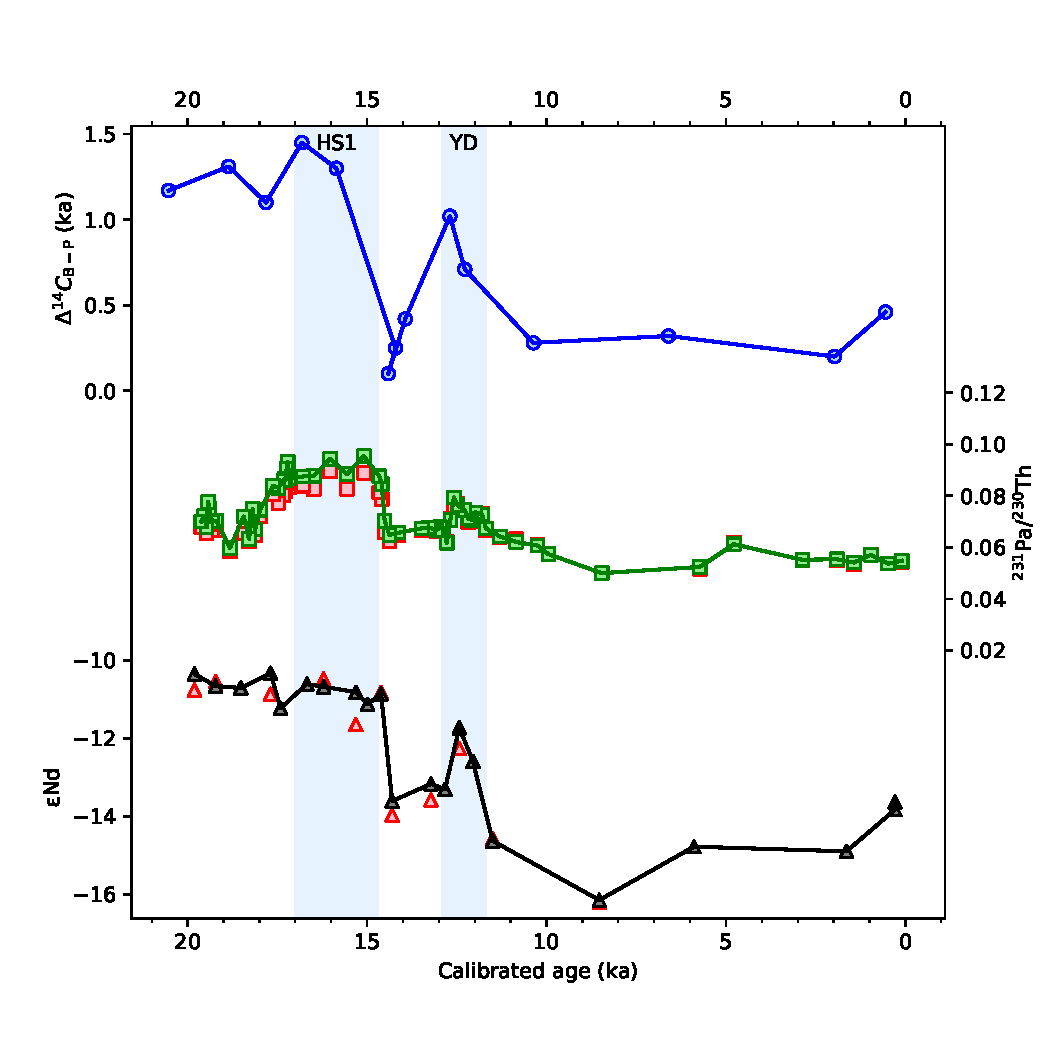
\includegraphics[width=\textwidth]{img/timeseries_B-P_PaTh_eNd}
    \caption{Time series of benthic--planktic foraminifera \fC{} ventilation age difference in OCE-326-GGC14 (top);
             \PaTh{} ratio in calculated against $^{238}$U (green) and $^{232}$U (red) OCE326-GGC5 core on Bermuda rise \parencite[data from][]{mcmanus2004collapse};
             Neodynium isotopic ratio excursion in unclean foraminifera (black) and reductively cleaned fish debris (red) from OCE326-GGC6 sediment core on Bermuda Rise (bottom) \parencite[data from][]{roberts2010synchronous}.}
            \label{fig:bp_path_end}
\end{figure}
The benthic--planktic foraminifera \fC{} offset (Figure \ref{fig:bp_path_end}, top) is considerably larger at LGM, HS1 and YD than during the BA and the Holocene.
Since \BP{} of a water mass effectively records the ventilation age (i.e. time since last exposure at the surface) \parencite{lynch2014tracers}, these results indicate that the North Atlantic was highly stratified during the cold periods, with younger northern sourced waters displaced in the deep ocean by the intrusion of more ancient waters of southern origin.
This supports evidence for the slowdown or shutoff of NADW formation during these cold periods, allowing Antarctic Bottom Water to fill the global abyssal basins \parencite{boyle1985comparison, bard1994north, thornalley2011deglacial}.
Likewise, the rapid rejuvenation of deep waters at the HS1--BA and YD--Holocene transitions shown in the \BP{} time series indicates rapid resumption of the contemporary (warm) mode ocean overturning circulation.

\subsection{Question 4}
\label{sec:Q2.4}
The \BP{} changes described in Section \ref{sec:Q2.3} are largely consistent with isotopic trends described in other studies, as depicted in Figure \ref{fig:bp_path_end}.
The ratio of $^{231}$P sequestered in marine sediments to the more quickly scavenged $^{230}$Th is an indicator of the residence time of the overlying water mass \parencite{lynch2014tracers}, and the high values recorded on the Bermuda rise for the HS1, and to a lesser extent YD, indicate poor export of $^{231}$P from the region during the postglacial stadials.
This can be explained by the arrest of the southward movement of NADW, as described above, with the steep \PaTh{} drop at \textapprox 15.5 marking the abrupt resumption of the AMOC following HS1 \parencite{mcmanus2004collapse}.
However, one issue with this using the particular proxy to infer changes in global circulation is that the distinction between a complete shutdown and a more moderate shift to a shallower, more locally confined circulation of North Atlantic waters is not always readily apparent, since the sedimentary \PaTh{} signal essentially records change in the entire column of water above \parencite{roberts2010synchronous}. 

Since $^{143}$Nd/$^{144}$Nd (\eNd{}) serves as a form of isotopic signature of different ocean mass sources, it can be used to supplement the interpretation of the other records in Figure \ref{fig:bp_path_end} \parencite{lynch2014tracers}. 
The high values from the LGM through to the end of HS1 provide evidence for the incursion of AABW into the Northwest Atlantic, with a marked shift to less radiogenic Northern-sourced waters following the YD, supporting the theory of AMOC modulation as a distinctive feature of deglacial climate change \parencite{roberts2010synchronous}.

\subsection{Question 5}
\label{sec:Q2.5}
\begin{figure}[h]
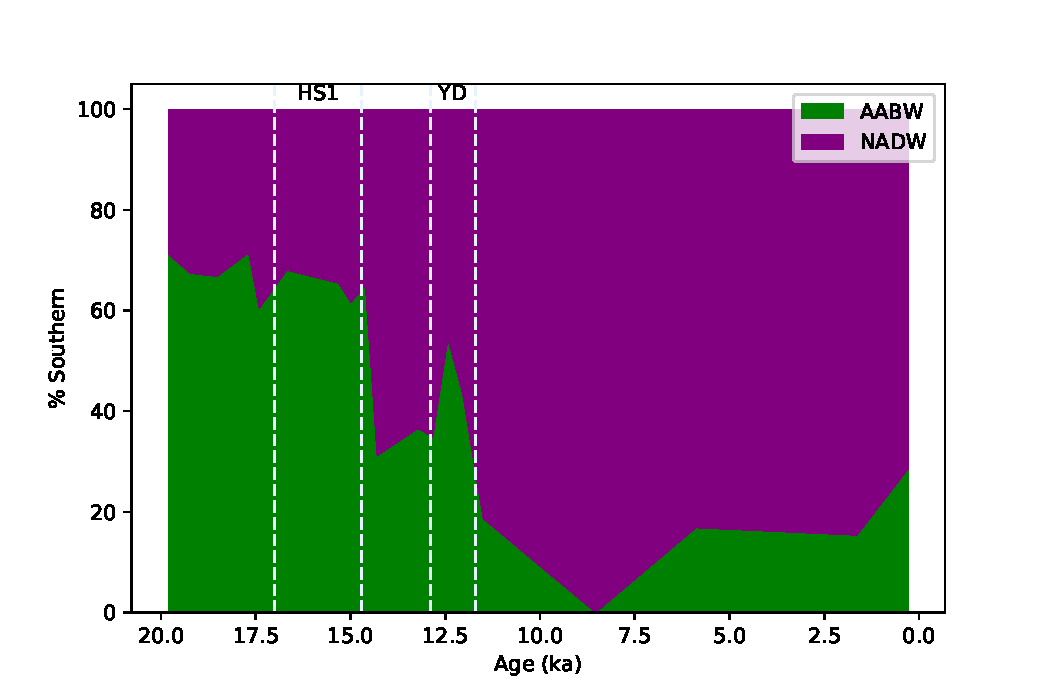
\includegraphics[width=\textwidth]{img/north_south}
    \caption{Proportion of northern (NADW) and southern (AABW) waters at Bermuda Rise , as estimated from unclean foraminifera \eNd{} in OCE326-GGC6 sediment core.}
    \label{fig:north_south}
\end{figure}


To visualise the varying influence of Northern and Southern sourced waters over the past 20 ka, an assumption is made that AABW (\eNd=$-8$ \parencite{garcia2014rare}) and NADW (\eNd=$-16.15$, lowest value in core) represent the two mixing end-members for the ocean mass bathing the Bermuda rise, as recorded in sediment core OCE326-GGC6.
The intrusion of southern sourced waters can clearly be seen in Figure \ref{fig:north_south}.
However, the exact values used here were chosen rather abitrarily from among a large range of observations for the \emph{present}, whereas values may have varied considerably over time, especially given that AABW, treated here as an opposing end-member to NADW, is in fact a product of Atlantic, Indian and Pacific waters which are likely to have mixed in different ratios in the past.
Futhermore, the dominant processes controlling water radiogenic properties may have changed.
This highlights the uncertainty introduced when certain ocean mass properties, such as \eNd{}, are assumed to be constant over time.
